\documentclass[11pt]{article}
%Gummi|065|=)

\usepackage{array}
\usepackage{graphicx}
\usepackage{tgschola}
\usepackage{algorithmic}
\usepackage{amssymb}
\usepackage{amsmath}
\DeclareMathOperator*{\argmax}{argmax}

\title{\textbf{SSU : Assignment 3} \\ \textbf{Digit recognition using Convolutional neural networks}}
\author{\textbf{Teymur Azayev}}
\date{}


\begin{document}

\maketitle

\section{Overview}
This document is a short report for the third assignment from the subject. It includes a theoretical overview of the task, an explanation of the implementation, results and a short discussion.

\section{Task}
The task is to train a small convolutional neural network on a commonly used dataset named MNIST.
This dataset consists of images of digits 0 to 9 inclusive.
We will first train the network on a subset of the dataset, namely digits 6 to 9 with various proportions,
noting the generalization accuracy after having trained on each proportion.
We will then train the network on the complete subset of digits 0 to 5 and then reuse the convolutional
layers for the training of digits 6 to 9, demonstrating the efficiency of transfer learning.

\section{Implementation and results} 
The convolutional neural network is implemented in python using tensorflow. The architecture is specified in the 
given task so it will not be mentioned here. We use a batchsize of 100 and an ADAM optimizer with an $\alpha$ of $0.001$. The network weights are initialized randomly with a standard deviation of $0.01$. Each configuration was trained 7 times for a total of 300 iterations and an average of the test accuracies is obtained. The following figure shows the result trained on the 6 to 9 digits with various proportions.


% Include image on raw 69 here
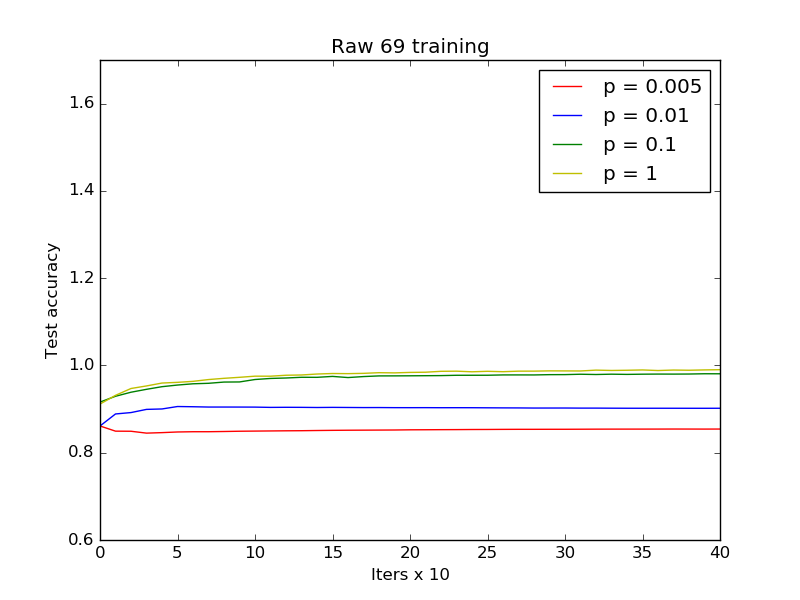
\includegraphics[width=\textwidth]{Raw69training}


The network is now trained on the 0 to 5 digits. We now freeze the convolutional layers (not allow gradients to flow through them) and retrain the network on digits 6 to 9. The following figure demonstrates the results \\ 


% Insert the retrained network results on the 6 to 9
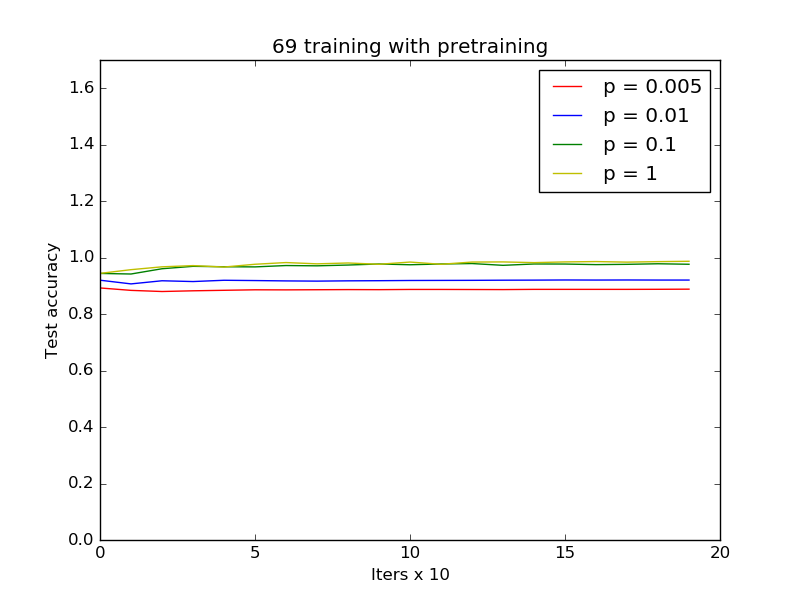
\includegraphics[width=\textwidth]{69trainingwithpretraining}

\section{Use of regularization}
We will now add the dropout technique to the fully connected layers of the network as a method of regularization.
A keep probability of 0.5 is used. 

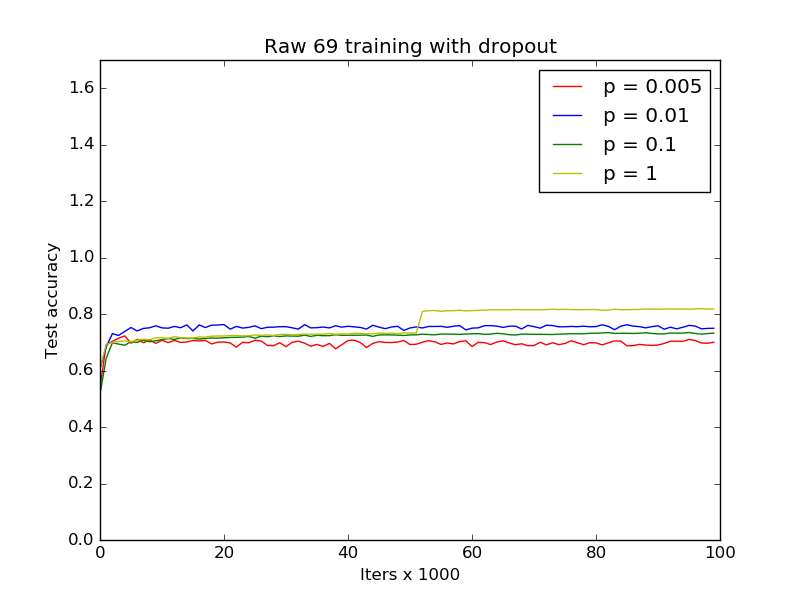
\includegraphics[width=\textwidth]{Raw69trainingwithdropout}

\section{Discussion}
We saw that using a higher proportion of data leads to smaller test error (better generalization). 
We also demonstrated the effectiveness of transfer learning where we used a network which was trained on 
one dataset as a feature extractor on top of which we trained another network. We can see that this 
method alleviates the need for large datasets which is a typical problem with deep learning.



\section{Conclusion}
This concludes the report on this task.


\end{document}
